% !TeX program = pdflatex
% =============================================================
% Public Economics -- Lecture 1
% Why Study Public Finance?
% Based on: Gruber, J. "Public Finance and Public Policy", Ch. 1
% Austrian institutional and empirical context added for WU Vienna.
% =============================================================
\documentclass[11pt,aspectratio=169]{beamer}

\usetheme{metropolis}
\usepackage[utf8]{inputenc}
\usepackage[T1]{fontenc}
\usepackage{lmodern}
\usepackage{booktabs}
\usepackage{array}
\usepackage{textcomp}
\usepackage{siunitx}
\usepackage{tikz}
\usepackage{pgfplots}
\pgfplotsset{compat=1.18}
\usetikzlibrary{positioning,arrows.meta,calc}

% ----------------------------------------------------------------
% Colors: WU Vienna blue as primary accent
% ----------------------------------------------------------------
\definecolor{wublue}{HTML}{003D7C}
\definecolor{wulight}{HTML}{4F8FC4}
\definecolor{wugray}{HTML}{5C6670}
\definecolor{wured}{HTML}{B0202E}
\setbeamercolor{palette primary}{bg=wublue,fg=white}
\setbeamercolor{frametitle}{bg=wublue,fg=white}
\setbeamercolor{progress bar}{fg=wublue,bg=wulight!30}
\setbeamercolor{alerted text}{fg=wured}

\setbeamertemplate{frame footer}{Why Study Public Finance?}
\setbeamertemplate{footline}[frame number]

\title{Public Economics}
\subtitle{Lecture 1 \(\cdot\) Why Study Public Finance?}
\author{Shushanik Margaryan}
\institute{WU Vienna University of Economics and Business}
\date{Winter Term}

% Source note command for footnote-style citations on data slides
\newcommand{\srcnote}[1]{{\footnotesize\color{wugray}Source: #1}}

\begin{document}

% =============================================================
\begin{frame}
  \titlepage
\end{frame}

% =============================================================
\begin{frame}{Today's Questions}
  \begin{itemize}
    \item What is \alert{public finance}, and what are the key questions the field addresses?
    \item What are the key facts about the size and growth of government, and the distribution of taxes and spending --- in the US, across the OECD, and here in \alert{Austria}?
    \item How do the questions of public finance show up in a concrete policy debate --- the Covid-19 pandemic?
  \end{itemize}
  \vspace{1em}
  \begin{block}{Based on}
    Gruber, J. \emph{Public Finance and Public Policy}, Ch.\ 1 --- ``Why Study Public Finance?''
  \end{block}
\end{frame}

% =============================================================
\begin{frame}{Outline}
  \tableofcontents
\end{frame}

% =============================================================
\section{A Motivating Case: Covid-19}

\begin{frame}{2020: A Natural Experiment in the Role of Government}
  \begin{columns}[T]
    \begin{column}{0.5\textwidth}
      \textbf{United States}
      \begin{itemize}
        \item GDP fell 31.2\% (Q2 2020); unemployment rose to 14.8\%
        \item \$2.2 trillion CARES Act (March 2020): direct payments, expanded UI, business loans
        \item States diverged sharply: strict lockdowns (CA, NY) vs.\ minimal restrictions (FL)
        \item Republicans vs.\ Democrats disagreed on \emph{almost every} dimension of the response
      \end{itemize}
    \end{column}
    \begin{column}{0.5\textwidth}
      \textbf{Austria}
      \begin{itemize}
        \item First EU country to enter a full nationwide lockdown (March 16, 2020)
        \item \emph{Kurzarbeit} (short-time work) massively expanded to prevent layoffs
        \item COVID-19 relief packages: Fixkostenzuschuss, Ausfallsbonus, Corona-Hilfsfonds
        \item Feb 2022: Austria became the \emph{first EU country} to legislate a general Covid-19 vaccination mandate
      \end{itemize}
    \end{column}
  \end{columns}
  \vspace{0.5em}
  \centering
  \alert{Every one of these decisions is a public finance decision.}
\end{frame}

% =============================================================
\section{1.1 The Four Questions of Public Finance}

\begin{frame}{What Is Public Finance?}
  \begin{block}{Public finance}
    The study of the role of \textbf{government} in the economy.
  \end{block}
  \vspace{1em}
  \textbf{The four questions of public finance:}
  \begin{enumerate}
    \item \textbf{When} should the government intervene in the economy?
    \item \textbf{How} might the government intervene?
    \item What is the \textbf{effect} of those interventions on economic outcomes?
    \item \textbf{Why} do governments choose to intervene in the way that they do?
  \end{enumerate}
\end{frame}

\begin{frame}{Q1: When Should the Government Intervene?}
  \textbf{Baseline:} in a competitive market, the equilibrium (supply = demand) maximizes the \emph{social efficiency} of trade.
  \begin{itemize}
    \item Every trade valued by both sides happens; no valuable trade is missed.
    \item So the free market is the benchmark --- government intervention needs a \emph{justification}.
  \end{itemize}
  \vspace{1em}
  \begin{alertblock}{Two justifications for intervention}
    \begin{enumerate}
      \item \textbf{Market failure} --- the market outcome is not efficient
      \item \textbf{Redistribution} --- society wants a different \emph{distribution} of the (efficient) outcome
    \end{enumerate}
  \end{alertblock}
\end{frame}

\begin{frame}{Market Failure: The Health Insurance Example}
  \begin{block}{Market failure}
    A problem that causes the market economy to deliver an outcome that does not maximize efficiency.
  \end{block}
  \begin{itemize}
    \item Health insurance \emph{looks} like a textbook competitive market: many buyers, many sellers.
    \item But: if I skip a flu shot, I raise \emph{my} risk of getting the flu --- and the risk that I infect \emph{you}.
    \item I only weigh \emph{my own} costs and benefits when deciding whether to insure/vaccinate; I ignore the cost I impose on others.
  \end{itemize}
  \vspace{0.5em}
  \centering
  $\Rightarrow$ a \textbf{negative externality}: private decisions $\neq$ socially efficient decisions.
\end{frame}

\begin{frame}{Application: Vaccines, Externalities, and Herd Immunity}
  \begin{itemize}
    \item US measles: vaccine (1963) cut cases from 3--4 million/year to under 3{,}000/year by the 1980s.
    \item 1989--91 resurgence (50{,}000+ cases) and a 2014--15 Disneyland outbreak were traced to \emph{unvaccinated} clusters.
    \item Response: California (2014) ended personal-belief exemptions for school enrollment --- vaccination rates rose sharply.
    \item Worldwide: 200{,}000 measles deaths in 2019, a 50\% rise in three years.
  \end{itemize}
  \begin{block}{The logic}
    Because an unvaccinated person imposes costs on others, private choices under-provide vaccination relative to the social optimum --- a textbook case for government intervention.
  \end{block}
\end{frame}

\begin{frame}{Austria's Case: The 2022 Covid-19 Vaccination Mandate}
  \begin{itemize}
    \item Feb 2022: Austria's \emph{Impfpflichtgesetz} made Covid-19 vaccination compulsory for adults --- a first in the EU.
    \item Justified explicitly on \textbf{externality} grounds: protecting the health system and others, not just oneself.
    \item June 2022: the \emph{Verfassungsgerichtshof} (Constitutional Court) upheld the law \emph{in principle}, but applied strict scrutiny because a vaccine mandate is a serious intervention in bodily autonomy.
    \item The mandate was never enforced with fines and was repealed in 2023 as Omicron changed the risk calculus.
  \end{itemize}
  \begin{alertblock}{Why this matters for public finance}
    A textbook market-failure argument (Q1) still had to survive constitutional \emph{and} political scrutiny (Q4) before becoming policy (Q2) --- and it was reversed once the underlying facts changed (Q3).
  \end{alertblock}
  \srcnote{Verfassungsgerichtshof, \textit{Impfpflichtgesetz} decisions G 29/2022, G 37/2022 (2022).}
\end{frame}

\begin{frame}{The Second Motive: Redistribution}
  \begin{block}{Redistribution}
    The shifting of resources from some groups in society to others.
  \end{block}
  \begin{itemize}
    \item Think of the economy as a \textbf{pie}: efficiency determines its \emph{size}.
    \item Society may also care about the \emph{distribution} of slices --- e.g., valuing \texteuro{}1 more to a poor household than to a rich one.
  \end{itemize}
  \vspace{0.5em}
  \begin{alertblock}{The equity--efficiency trade-off}
    Redistribution usually changes behavior (e.g., work incentives), which can \emph{shrink the pie} even as it changes how it is sliced.
  \end{alertblock}
\end{frame}

\begin{frame}{Why Redistribution Is on the Table in Austria}
  \begin{columns}[T]
    \begin{column}{0.55\textwidth}
      \textbf{Income inequality}
      \begin{itemize}
        \item Gini coefficient (equivalized disposable income): 30.7 in 2021, up from 29.8 in 2020
        \item At-risk-of-poverty rate: \(\approx\) 12--14\% of the population
        \item Material deprivation nearly doubled: 201{,}000 people (2.3\%) in 2022 $\to$ 336{,}000 (3.7\%) in 2023
      \end{itemize}
    \end{column}
    \begin{column}{0.45\textwidth}
      \textbf{Wealth inequality}
      \begin{itemize}
        \item Median household net wealth: \(\approx\) \texteuro{}83{,}000
        \item Top 1\% hold roughly 40\%+ of total net wealth
        \item Bottom 50\% hold under 4\% of total net wealth
      \end{itemize}
    \end{column}
  \end{columns}
  \vspace{0.5em}
  \srcnote{Statistik Austria, EU-SILC (2023); Oesterreichische Nationalbank, Household Finance and Consumption Survey (HFCS).}
\end{frame}

\begin{frame}{Q2: How Might the Government Intervene?}
  Four broad policy tools:
  \begin{enumerate}
    \item \textbf{Tax or subsidize} private sale/purchase (change the price)
    \item \textbf{Restrict or mandate} private sale/purchase (change the quantity directly)
    \item \textbf{Public provision} (the government produces the good itself)
    \item \textbf{Public financing of private provision} (government pays; private firms produce)
  \end{enumerate}
\end{frame}

\begin{frame}{The Four Tools, With US and Austrian Examples}
  \begin{center}
  \small
  \begin{tabular}{@{}p{2.7cm}p{4.7cm}p{4.7cm}@{}}
    \toprule
    \textbf{Tool} & \textbf{US example} & \textbf{Austrian example} \\
    \midrule
    Tax/subsidize & ACA premium tax credits for low-income buyers & \emph{Pendlerpauschale} (commuter tax deduction); CO\textsubscript{2} pricing under the eco-social tax reform \\[0.3em]
    Mandate/restrict & ACA individual mandate (since repealed) & Covid-19 vaccination mandate (2022, repealed 2023) \\[0.3em]
    Public provision & Medicare (elderly), VA hospitals & ÖGK public health insurance; public hospitals (KAV/Gemeindespital network) \\[0.3em]
    Public financing of private provision & Medicare Part D (private insurers, public funds) & Social-insurance reimbursement of private physicians and private hospitals \\
    \bottomrule
  \end{tabular}
  \end{center}
\end{frame}

\begin{frame}{Q3: What Are the Effects of Interventions?}
  \begin{block}{Direct effects}
    What would happen \emph{if people did not change their behavior}.
  \end{block}
  \begin{block}{Indirect effects}
    What happens \emph{because} people change their behavior in response.
  \end{block}
  \vspace{0.5em}
  \textbf{Worked example (Gruber):} covering the uninsured in the 2010 US\\
  \begin{itemize}
    \item 49 million uninsured \(\times\) \$2{,}500/year \(\Rightarrow\) direct cost \(\approx\) \$125 billion
    \item If half of the privately insured \emph{drop} their coverage to join the free public plan: cost triples to \(\approx\) \$340 billion
    \item If only 10\% drop coverage: cost rises to \(\approx\) \$165 billion
  \end{itemize}
  \centering
  \alert{The indirect effect --- how people respond --- is an empirical question, and it is often the whole ballgame.}
\end{frame}

\begin{frame}{Application: Independent Scorekeepers}
  Answering Q3 requires credible, nonpartisan empirical analysis.
  \begin{columns}[T]
    \begin{column}{0.5\textwidth}
      \textbf{United States: the CBO}
      \begin{itemize}
        \item Congressional Budget Office (est.\ 1975)
        \item ``Scores'' the cost of every major bill before it can pass
        \item Its 2017 estimate (30M+ more uninsured under ACA repeal) helped sink the repeal effort
      \end{itemize}
    \end{column}
    \begin{column}{0.5\textwidth}
      \textbf{Austria: the Fiskalrat \& Budgetdienst}
      \begin{itemize}
        \item \emph{Fiskalrat} monitors compliance with EU and national fiscal rules
        \item Parliament's \emph{Budgetdienst} independently costs and analyzes budget bills for MPs
        \item Both flagged the 2024 deficit overshoot well before the official numbers were finalized
      \end{itemize}
    \end{column}
  \end{columns}
\end{frame}

\begin{frame}{Q4: Why Do Governments Do What They Do?}
  \begin{itemize}
    \item Q2 was \textbf{normative} (how \emph{should} government intervene?). Q4 is \textbf{positive} (why do governments actually behave as they do?).
    \item Governments aggregate the preferences of millions of citizens --- imperfectly.
    \item Just as markets can fail, \textbf{governments can fail} too: policy can reflect lobbying, electoral incentives, or institutional constraints rather than pure efficiency or equity goals.
  \end{itemize}
  \begin{alertblock}{Political economy}
    The theory of how the political process produces decisions that affect individuals and the economy.
  \end{alertblock}
  \centering
  Same virus, same facts, very different policies in the US, Canada, Germany, the UK --- and across Austria's own coalition governments.
\end{frame}

% =============================================================
\section{1.2 Facts on Government: US, OECD, and Austria}

\begin{frame}{Why Look at the Facts?}
  \begin{itemize}
    \item Public finance is compelling because government is \emph{everywhere} in economic life.
    \item We now look at five facts: size, decentralization, deficits/debt, spending composition, and revenue composition.
    \item For each, we compare the textbook US numbers to \textbf{Austria and the OECD} --- the environment you will actually work and pay taxes in.
  \end{itemize}
\end{frame}

\begin{frame}{Fact 1: The Size of Government Has Grown --- Everywhere}
  \begin{itemize}
    \item US federal spending: 3.4\% of GDP (1930) \(\to\) \(\approx\)50\% of GDP (1944, WWII peak) \(\to\) \(\approx\)20\% of GDP (recent decades)
    \item Growth has been even faster in many other OECD countries since 1960
    \item Greece: government share roughly tripled since 1960; Sweden peaked near two-thirds of GDP in the early 1990s
  \end{itemize}
  \begin{block}{Discussion}
    What explains the twentieth-century growth of government spending across almost every developed country?
  \end{block}
\end{frame}

\begin{frame}{Austria Today: One of the Largest Governments in the EU}
  \begin{center}
  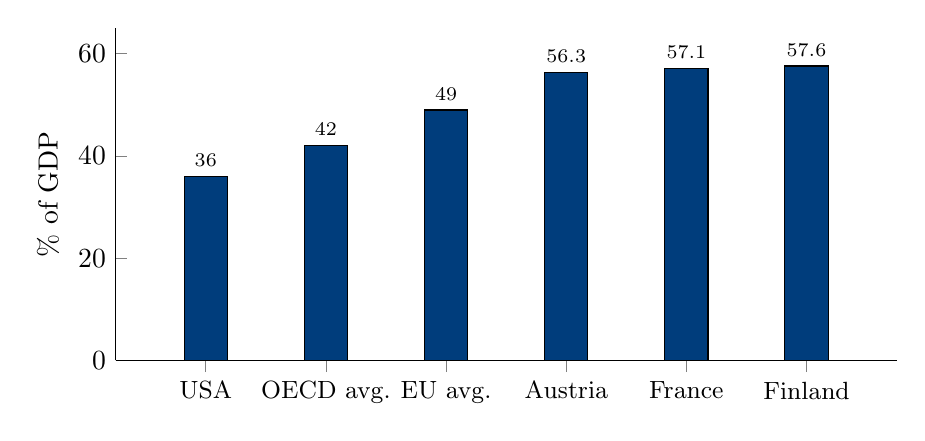
\begin{tikzpicture}
    \begin{axis}[
      ybar, bar width=0.55cm,
      width=11.5cm, height=5.8cm,
      ymin=0, ymax=65,
      symbolic x coords={USA,OECD avg.,EU avg.,Austria,France,Finland},
      xtick=data,
      x tick label style={font=\small},
      ylabel={\% of GDP},
      nodes near coords,
      nodes near coords style={font=\scriptsize},
      enlarge x limits=0.15,
      axis lines*=left,
      ]
      \addplot[fill=wublue] coordinates {
        (USA,36) (OECD avg.,42) (EU avg.,49) (Austria,56.3) (France,57.1) (Finland,57.6)
      };
    \end{axis}
  \end{tikzpicture}
  \end{center}
  \vspace{-0.3em}
  \centering \small
  Austria had the \textbf{3rd-highest} total government spending ratio (``Staatsquote'') in the EU in 2024.\\
  \srcnote{Eurostat; Statistik Austria (2024); OECD Government at a Glance.}
\end{frame}

\begin{frame}{Fact 2: Decentralization --- Who Spends, Who Taxes?}
  \textbf{United States:} the federal government provides the majority of spending, but state/local spending is still \(>\)40\% of total government spending (\(>\)17\% of GDP).
  \vspace{1em}
  \begin{alertblock}{Austria's federalism paradox}
    \begin{itemize}
      \item \textbf{Bund} (federal): collects \(\approx\)72\% of tax revenue, but does only \(\approx\)48\% of spending
      \item \textbf{Länder}: collect \(\approx\)12\% of tax revenue, but do \(\approx\)31\% of spending
      \item \textbf{Gemeinden} (municipalities): collect \(\approx\)12\% of tax revenue, but do \(\approx\)25\% of spending
    \end{itemize}
  \end{alertblock}
  \centering \small
  Revenue-raising power and spending responsibility are separated --- a classic ``who pays vs.\ who decides'' problem in fiscal federalism.\\
  \srcnote{Agenda Austria, fiscal federalism analysis; Austrian \emph{Finanzausgleich}.}
\end{frame}

\begin{frame}{Fact 3: Deficits and Debt}
  \begin{block}{Definitions}
    \textbf{Deficit} = spending $-$ revenue in a given year. \quad \textbf{Debt} = accumulated past deficits.
  \end{block}
  \begin{itemize}
    \item US: near balance for decades (excl.\ WWII), large deficits since the 1970s--80s; debt now above 100\% of GDP.
    \item State/local governments in the US are typically required to balance their budgets --- and mostly do.
  \end{itemize}
\end{frame}

\begin{frame}{Austria vs.\ the Maastricht Rules}
  \begin{center}
  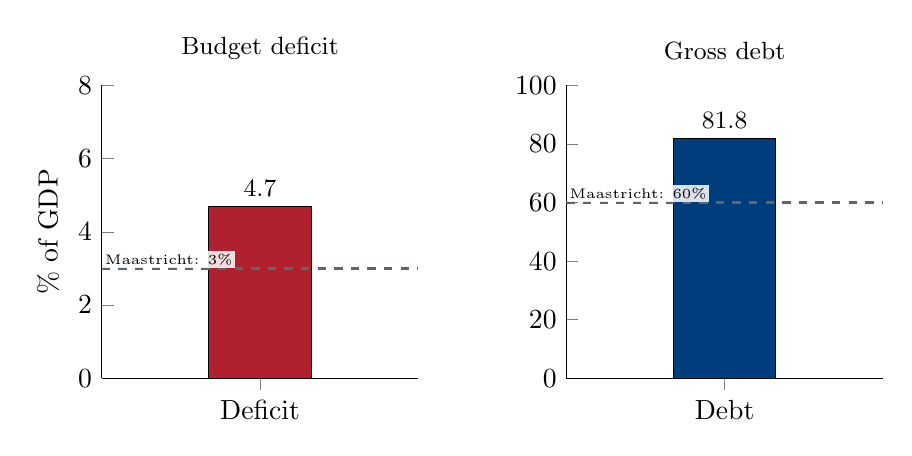
\begin{tikzpicture}
    \begin{axis}[
      ybar, bar width=1.3cm,
      width=5.6cm, height=5.3cm,
      ymin=0, ymax=8,
      symbolic x coords={Deficit},
      xtick=data,
      ylabel={\% of GDP},
      title={Budget deficit},
      title style={font=\small},
      nodes near coords,
      nodes near coords style={font=\small},
      enlarge x limits=1.3,
      axis lines*=left,
      ]
      \addplot[fill=wured] coordinates {(Deficit,4.7)};
      \draw[dashed, thick, wugray] (rel axis cs:0,0.375) -- (rel axis cs:1,0.375);
      \node[anchor=south west, font=\tiny, fill=white, fill opacity=0.85, text opacity=1, inner sep=1pt]
        at (rel axis cs:0,0.375) {Maastricht: 3\%};
    \end{axis}
    \begin{axis}[
      at={($(5.9cm,0)$)},
      ybar, bar width=1.3cm,
      width=5.6cm, height=5.3cm,
      ymin=0, ymax=100,
      symbolic x coords={Debt},
      xtick=data,
      title={Gross debt},
      title style={font=\small},
      nodes near coords,
      nodes near coords style={font=\small},
      enlarge x limits=1.3,
      axis lines*=left,
      ]
      \addplot[fill=wublue] coordinates {(Debt,81.8)};
      \draw[dashed, thick, wugray] (rel axis cs:0,0.6) -- (rel axis cs:1,0.6);
      \node[anchor=south west, font=\tiny, fill=white, fill opacity=0.85, text opacity=1, inner sep=1pt]
        at (rel axis cs:0,0.6) {Maastricht: 60\%};
    \end{axis}
  \end{tikzpicture}
  \end{center}
  \centering \small
  Austria 2024: deficit \textbf{4.7\%} of GDP, gross debt \textbf{81.8\%} of GDP --- both above their Maastricht ceilings (3\% and 60\%).\\
  \srcnote{Statistik Austria, Maastricht notification (2025); BMF, Öffentliche Schulden 2024.}
\end{frame}

\begin{frame}{Discussion: Deficits and Debt}
  \begin{itemize}
    \item What are the costs of running larger deficits and carrying more debt?
    \item Why might it make sense to let deficits rise in \emph{some} years (recessions, pandemics) even under fixed fiscal rules?
    \item Austria's Länder and Gemeinden are far closer to balanced budgets than the Bund --- why might that be, given Fact 2?
  \end{itemize}
\end{frame}

\begin{frame}{Fact 4: What Does Government Spend On?}
  \textbf{US federal budget, then and now:} defense fell from \(\approx\)half of spending (1960) to under one-sixth today; Social Security (\(\approx\)19\%) and health programs (\(\approx\)30\%) grew to take its place.
  \begin{block}{Public goods vs.\ social insurance}
    Defense is a classic \textbf{public good} (non-excludable, non-rival benefit). Pensions and health coverage are \textbf{social insurance}: government provision of insurance where private insurance markets under-perform.
  \end{block}
\end{frame}

\begin{frame}{Austria's Social Spending}
  \begin{center}
  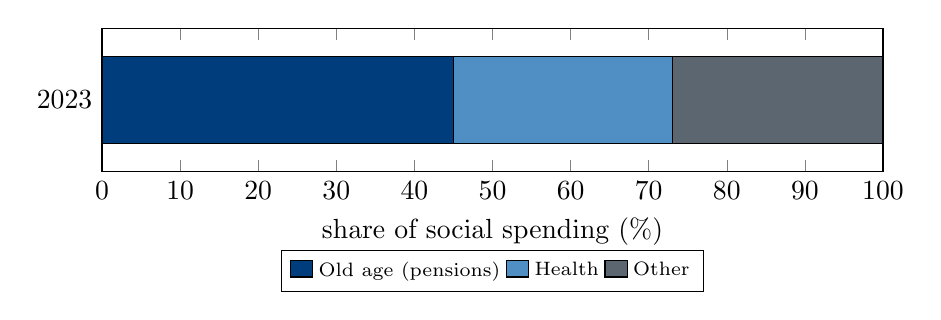
\begin{tikzpicture}
    \begin{axis}[
      xbar stacked, bar width=1.1cm,
      width=11.5cm, height=3.4cm,
      xmin=0, xmax=100,
      symbolic y coords={2023},
      ytick=data,
      xlabel={share of social spending (\%)},
      legend style={at={(0.5,-0.55)},anchor=north,legend columns=3,font=\scriptsize},
      enlarge y limits=1,
      ]
      \addplot[fill=wublue] coordinates {(45,2023)};
      \addplot[fill=wulight] coordinates {(28,2023)};
      \addplot[fill=wugray] coordinates {(27,2023)};
      \legend{Old age (pensions), Health, Other}
    \end{axis}
  \end{tikzpicture}
  \end{center}
  \centering \small
  ``Other'' = family benefits, unemployment insurance, disability, and housing support.\\
  Total social spending: \texteuro{}146.2 billion (2023). Austria's \textbf{Sozialquote}: 30.9\% of GDP --- among the highest social-spending ratios in the world.\\
  \srcnote{Statistik Austria, ESSPROS social protection statistics (2023).}
\end{frame}

\begin{frame}{Fact 5: Where Does the Revenue Come From?}
  \textbf{United States:} individual income tax (\(\approx\)half of federal revenue) has stayed roughly constant; corporate tax fell from \(\approx\)25\% to \(\approx\)6\% of revenue; payroll taxes rose from one-sixth to over one-third.
  \begin{block}{Discussion}
    What are the implications of shifting the tax burden from businesses and consumption toward workers' earnings?
  \end{block}
\end{frame}

\begin{frame}{Austria's Tax Mix: Heavy on Labor}
  \begin{itemize}
    \item VAT (\emph{Umsatzsteuer}): \(\approx\)\texteuro{}35.4 billion (2022) --- the single largest tax
    \item Wage tax (\emph{Lohnsteuer}): \(\approx\)\texteuro{}25 billion --- about one-sixth of total tax revenue
    \item Corporate tax (\emph{Körperschaftsteuer}): \(\approx\)\texteuro{}7.8 billion --- only 2.2\% of GDP
    \item VAT + wage tax alone \(\approx\) two-thirds of all tax revenue
  \end{itemize}
  \begin{alertblock}{A distinctive feature}
    Austria taxes \textbf{labor} more heavily, relative to the size of its economy, than any other EU country --- while capital and consumption taxes play a comparatively smaller role.
  \end{alertblock}
  \srcnote{Agenda Austria; Bundesministerium für Finanzen (BMF), tax revenue statistics (2022--24).}
\end{frame}

\begin{frame}{Fact 6: The Regulatory State}
  Beyond taxing and spending, governments \textbf{regulate}.
  \begin{center}
  \small
  \begin{tabular}{@{}lll@{}}
    \toprule
    \textbf{Domain} & \textbf{United States} & \textbf{Austria} \\
    \midrule
    Food \& drug safety & FDA & AGES (Agentur für Gesundheit) \\
    Workplace safety & OSHA & Arbeitsinspektorat, AUVA \\
    Environment & EPA & Umweltbundesamt \\
    Communications & FCC & RTR (Rundfunk und Telekom Regulierungs-GmbH) \\
    \bottomrule
  \end{tabular}
  \end{center}
  \vspace{0.5em}
  \centering
  Regulatory agencies can be tiny in budget (the FDA is \(<\)0.025\% of the US budget) yet govern a huge share of everyday economic life.
\end{frame}

% =============================================================
\section{1.3 Back to Covid-19: The Four Questions in Practice}

\begin{frame}{The Four Questions, Applied}
  \begin{enumerate}
    \item \textbf{When intervene?} Mask mandates, business closures, and vaccine mandates were all justified by \emph{externalities} --- exactly the logic of the flu-shot and measles examples.
    \item \textbf{How intervene?} Compare Kurzarbeit (public financing of private employment) to US direct payments and PPP loans (public financing of private provision).
    \item \textbf{What effect?} Hundreds of NBER working papers (23.8\% of all 2020 output) tried to measure whether lockdowns, PPP, and UI expansions actually changed behavior.
    \item \textbf{Why this policy?} Democrats and Republicans proposed very different follow-up packages \emph{using the same evidence} --- and Austria's own coalition partners split over mandate enforcement.
  \end{enumerate}
\end{frame}

% =============================================================
\section{1.4 Conclusion}

\begin{frame}{Highlights}
  \begin{itemize}
    \item Government intervention is justified by \textbf{market failure} (grow the pie) or \textbf{redistribution} (reslice the pie) --- not simply by good intentions.
    \item There are many tools to intervene: taxes/subsidies, mandates/restrictions, public provision, and public financing of private provision.
    \item Empirical public finance --- direct vs.\ indirect effects --- is essential to judging \emph{how well} any policy actually works.
    \item Governments can fail too: political economy explains why actual policy often departs from the efficiency/equity ideal.
    \item Government in Austria is large by international standards (56.3\% of GDP), fiscally federal in a distinctive way, and its tax base leans heavily on labor income.
  \end{itemize}
\end{frame}

\begin{frame}{Discussion Questions for Next Time}
  \begin{enumerate}
    \item Is Austria's heavy reliance on labor taxation (vs.\ capital/consumption) efficient, equitable, both, or neither?
    \item Austria's Bund raises 72\% of tax revenue but does only 48\% of spending. What are the risks of this mismatch between taxing and spending authority?
    \item Consider the case for a wealth tax in a country where the top 1\% hold \(\approx\)40\% of net wealth. Frame your answer using the equity--efficiency trade-off.
    \item Was the 2022 Covid-19 vaccination mandate a case of correcting a market failure, or a case of government overreach? Use the four questions of public finance to structure your answer.
  \end{enumerate}
\end{frame}

\begin{frame}{Sources}
  \small
  \textbf{Textbook:} Gruber, J. \emph{Public Finance and Public Policy}, Ch.\ 1, Worth Publishers.
  \vspace{0.5em}

  \textbf{Austrian and international data:}
  \begin{itemize}
    \item Statistik Austria: Staatsausgaben nach Aufgabenbereichen; Sozialquote/ESSPROS; EU-SILC income and living conditions
    \item Bundesministerium für Finanzen (BMF): Öffentliche Schulden 2024; tax revenue statistics
    \item Parlament Österreich, Budgetdienst: Gebarungserfolg und gesamtstaatliche Entwicklung 2024
    \item Oesterreichische Nationalbank (OeNB): Household Finance and Consumption Survey (HFCS)
    \item Agenda Austria: Staatsquote, fiscal federalism, and tax-structure analyses
    \item Eurostat; OECD \emph{Government at a Glance}
    \item Verfassungsgerichtshof: \emph{Impfpflichtgesetz} decisions G 29/2022, G 37/2022
  \end{itemize}
\end{frame}

\begin{frame}[standout]
  Thank you!\\
  \vspace{0.5em}
  \small Questions and discussion
\end{frame}

\end{document}
